\documentclass{article}
\usepackage{tikz}
\usetikzlibrary{angles, quotes}
\usepackage{amssymb}
\usepackage{pgfplots}
\pgfplotsset{width=10cm,compat=1.9}
\usepgfplotslibrary{statistics}
\usepackage[left=2.54cm,right=2.54cm,top=2.54cm,bottom=2.54cm]{geometry}
\usepackage{tasks} %Paquete necesario para la producción de items horizontales para algunos ejercicios de tarea empleando el comando /begin{multicols}}{#}.../end{multicols} para ayudarnos a reducir las páginas
\usepackage{pdflscape} %comando que permite cambiar a orientación horizontal las hojas%
\usepackage{soul} %Paquete para permitir la compilación de acentos usando el comando {\hl{}}}\\
\sethlcolor{yellow(munsell)} %comando para definir el color para el subrayado usando el comando \hl
\usepackage[utf8]{inputenc}
\usepackage[spanish]{babel}
\usepackage{icomma}
\usepackage{ragged2e}		
\usepackage{siunitx}
\usepackage{url}
\usepackage[colorlinks=true, urlcolor=blue,  linkcolor=Cerulean, citecolor=green]{hyperref}
\usepackage{pdfpages}
\usepackage{blindtext} %Paquete que genera texto ficticio (dummy text) con el comando: \blindtext
\usepackage{cancel} %in the preamble gives you four different modes of striking through: \cancel{text to cancel} draws a diagonal line (slash) through its argument, \bcancel{text to cancel} uses the negative slope (a backslash), \xcancel{text to cancel} draws an X (actually \cancel plus \bcancel), \cancelto{〈value〉}{〈expression〉} draws a diagonal arrow through the 〈expression〉pointing to the 〈value〉 (math-mode only)
\usepackage{csquotes}
\usepackage{afterpage}
\usepackage{parskip} 
\usepackage{float}
\usepackage{enumitem}
%\usepackage{multicol}%Paquete que permite la creación aislada de columnas de texto. De esta forma se reduce la cantidad de páginas en nuestro documento
\usepackage{lipsum} %Paquete que genera texto de relleno al igual que \usepackage{blindtext}, se usa con el comando \lipsum[#-#] los #(hashtags) delimitan el número de páginas que deseamos ocupar del paquete lipsum para usarlos como relleno. 

% Definir el comando personalizado para la nota
\newcommand{\mynote}[1]{%
\begin{tikzpicture}[baseline=-0.75ex]
\node[draw, circle, fill=Apple Green!60, inner sep=2pt] (note) {\textbf{Nota:}};
\end{tikzpicture}%
\ \textit{#1}%
}

% Definición de comandos para variables con barra
\newcommand{\xbar}{\overline{x}}
\newcommand{\ybar}{\overline{y}}

\newenvironment{Figura}
{\par\medskip\noindent\minipage{\linewidth}}
{\endminipage\par\medskip}
\usepackage{caption}
\usepackage[
backend=biber,
sorting=none,
url=true
]{biblatex} %bibliografía
\addbibresource{biblio.bib}
% Establecer el espacio entre las entradas de la bibliografía
\setlength{\bibitemsep}{1\baselineskip} % Puedes ajustar el valor según tus preferencias
\usepackage{amsmath,amsthm,amssymb,amsfonts}
\usepackage{pifont} %Permite la compilación del comando \xmark: es el símbolo de la tachita
\usepackage{mathtools} %permite la compilación de símbolos para matrices
\usepackage{empheq} %Paquete que se relaciona con \usepackage[most]{tcolorbox} para la creación de cuadros/cajas de colores para delimitar los resultados matemáticos o líneas de texto usando la línea de comando: \begin{empheq}[box={\mymath[colback=orange(webcolor)!70,drop lifted shadow]}]{equation*} \end{empheq}
\usepackage[most]{tcolorbox} %Paquete que se relaciona con \usepackage{empheq} para la creación de cuadros/cajas de colores para delimitar los resultados matemáticos o líneas de texto
\renewcommand{\qedsymbol}{$\blacksquare$}
\usetikzlibrary{positioning,decorations.pathreplacing} %Paquete que permite la compilación de llaves para cuadros sinópticos (brace diagram) 
\usepackage{schemata} %The schemata package is designed just for these brace diagrams
\usepackage{booktabs}

\newcommand\AB[2]{\schema{\schemabox{#1}}{\schemabox{#2}}} %comando o paquete necesario para crear cuadros sinópticos

\newtcbox{\mymath}[1][]{%
nobeforeafter, math upper, tcbox raise base,
enhanced, colframe=blue!30!black,
colback=blue!30, boxrule=1pt,
#1} %Comando importante para encasillar los resultados matemáticos en cajas de diferentes colores, se relaciona con los paquetes \usepackage{empheq} y \usepackage[most]{tcolorbox} 

\newenvironment{sysmatrix}[1]
{\left(\begin{array}{@{}#1@{}}}
{\end{array}\right)}
\newcommand{\ro}[1]{%
\xrightarrow{\mathmakebox[\rowidth]{#1}}%
}
\newlength{\rowidth}% row operation width
\AtBeginDocument{\setlength{\rowidth}{3em}}  %Comando importante para laproducción de lineas de operaciones entre matrices, método de Gauss o Gauss Jordan se relaciona con \newenvironment{sysmatrix}

%formato para cambiar el horario a español
\usepackage[spanish]{datetime2}
\DTMsetdatestyle{spanish}

\renewcommand{\today}{\DTMdisplaydate{\the\year}{\the\month}{\the\day }{-1}}
%%%%%%%%%%%%%%%%%%%%%%%%%%%%%%%%%%%%%%%%%

\usepackage{datetime}
\newcommand{\mycurrenttime}{\xxivtime}

%%%%%%%%%%%%%%%%%%%%%%%%%%%%%%%%%%%%%%%%%%%%%%%%%%%%%%%%%%%%%%%%%%%%%%%%%%%%%%%%%%%%%%%%%%%%%%%%%%%%%%%%%%%%%%%%%%%%%%%%%%%%%%%%%%%%%%%%%%%%%%%%%


%%%%%%%%%%%%%Caja de color para el título%%%%%%%%%%%%%%%%%%%%%%%%%%%%%%%%%%%%%%%%%%%%%%%%%%%%%%

\definecolor{myframecolor}{RGB}{1, 45, 75} % Prussian Blue
\definecolor{myboxcolor}{RGB}{0, 107, 92} % Apple Green

\newtcolorbox{mybox}{
enhanced,
colback=myboxcolor!7, % Color de fondo del cuadro
colframe=myframecolor, % Color del marco del cuadro
arc=0pt,
boxrule=1pt,
borderline west={2mm}{-10mm}{myframecolor}, % Borde en el lado izquierdo
sharp corners=southwest,
width=\linewidth,
before=\par\vspace{\bigskipamount}, % Espacio antes del cuadro
after=\par\vspace{\bigskipamount} % Espacio después del cuadro
}

%%%%%%%%%%%%%%%%%%%%%%%%%%%%%%%%%%%%%%%%%%%%%%%%%%%%%%%%%Nueva caja%%%%%%%%%%%%%%%%%%%%%%%%%%%%%%%%%%%%%%%%%%%%%%%%%%%%%%%%%%%%%%%%%

\newtcolorbox{mybox2}{
enhanced,
colback=Apple Green!7, % Color de fondo del cuadro
colframe=Apple Green, % Color del marco del cuadro
arc=0pt,
boxrule=1pt,
borderline west={2mm}{-10mm}{Apple Green}, % Borde en el lado izquierdo
sharp corners=southwest,
width=\linewidth,
before=\par\vspace{\bigskipamount}, % Espacio antes del cuadro
after=\par\vspace{\bigskipamount} % Espacio después del cuadro
}


\newcommand{\euler}{e} %Comando para producir letra e de euler
\newenvironment{remark}{\par\vfill\footnotesize % Vertical white space above the remark and smaller font size
\begin{list}{}{
	\leftmargin=80pt % Indentation on the left
	\rightmargin=60pt}\item\ignorespaces % Indentation on the right
\makebox[-2.5pt]{\begin{tikzpicture}[overlay]
		\node[draw=Horizon!60,line width=2.5pt,circle,fill=Horizon!25,font=\sffamily\bfseries,inner sep=4pt,outer sep=0pt] at (-19pt,5pt){\textcolor{Horizon}{Nota}};\end{tikzpicture}} % Blue Nota in a circle
\advance\baselineskip -1pt}{\end{list}\vskip5pt} % Tighter line spacing and white space after remark
\usepackage{graphicx}

\usepackage{titling}

\input{colores.tex}

%%Producir signos de cita textual``Asignatura''

\newcommand{\xmark}{\ding{55}} %%%comando que genera la tachita

\newenvironment{MyColorPar}[1]{%
\leavevmode\color{#1}\ignorespaces%
}{%
}%

%%%%%%%%%%%%%%%%%%% Título de la tarea, Nombre de alumno

\title{ \textcolor{Sun}{\textbf{Ejercicios}}}
\author{\emph{Tarea} $\boldsymbol{\mid}$ \textcolor{Tarawera}{\textbf{Oscilaciones de la red}}}
\date{\today}

%%%%%%%%%%%%%%%%%%% Datos de la Materia

\usepackage{fancyhdr}
\fancypagestyle{plain}{%  the preset of fancyhdr 
\fancyhf{} % clear all header and footer fields
\fancyfoot[R]{
\includegraphics[width=2cm]{LogoFCFMBUAP (1).png}}
\fancyfoot[L]{{\bfseries{\thedate{}}} a las {\bfseries{\mycurrenttime{}}} horas{} (GMT-6, H. Puebla de Zaragoza, Pue)}
\fancyhead[L]{\textbf{Asignatura:} Estado Sólido}
\fancyhead[R]{\theauthor}
}
\makeatletter
\def\@maketitle{%
\newpage
\null%
\begin{center}%
\let \footnote \thanks
{\LARGE \@title \par}%
\vskip 1em%
%{\large \@date}%
\end{center}%
}
\makeatother

\usepackage{lipsum}  
\usepackage{cmbright}


%%%%%%%%%%%%%%%%%%%%%%%%%%%%%%%%%%%%%%%%%%%%%%%%%%%%%%%%%%%%%%%%%%%%%%%%%%%%%%%%%%%%%%%%%%%%%%%%%%%%%%%%%%%%%%%%%%%%%%%%%%%%%%%%%%%%%%%%%%%%%%%%%%%%%%%%%%%%%%%%%%%%%%%%%%%%%%%%%%%%%%%%%%%%%%%%%%%%%%

% Por si el color se llama "Apple Green" con espacio en colores.tex:
\colorlet{AppleGreen}{Apple Green}

% Caja AppleGreen con tono ajustable
\newenvironment{AGbox}[1][7]% 7 = tono por defecto (más grande => más claro)
{%
  \begin{tcolorbox}[
    enhanced, breakable,
    colframe=AppleGreen,
    colback=AppleGreen!#1,
    boxrule=1pt,
    borderline west={2mm}{-10mm}{AppleGreen},
    sharp corners=southwest,
    left=14pt,right=14pt,top=10pt,bottom=10pt,
     boxsep=6pt,
  ]%
}{%
  \end{tcolorbox}%
}


\begin{document}



\maketitle

%%%%%%%%%%%%%%%%%%% Datos del profesor, campus, aula e integrantes

\begin{mybox2}
\noindent
\begin{tabular}{@{}p{3.7cm}p{10.4cm}@{}}
\textbf{Profesor} & Dra. Ana Lilia González Ronquillo \\[3pt]
\textbf{Campus / Facultad} & \textcolor{prussianblue}{\textbf{C.U. BUAP}} / \textcolor{trueblue}{\textbf{FCFM}} \\[3pt]
\textbf{Edificio / Salón} & \textcolor{prussianblue}{\textbf{FM9}} / \textcolor{trueblue}{\textbf{301}} \\[6pt]
\textbf{Alumno} & Julio Alfredo Ballinas García
\end{tabular}
\end{mybox2}
\vspace{1cm}


\vspace{0.5cm}
\begin{center}
\begin{tikzpicture}
	% Dibuja círculos rellenos en diferentes colores
	\fill[bittersweet] (0,0) circle (0.17cm);
	\fill[Apple Green] (0.6,0) circle (0.17cm);
	\fill[trueblue] (1.2,0) circle (0.17cm);
	\fill[Aguamarina] (1.8,0) circle (0.17cm);
	\fill[Sun] (2.4,0) circle (0.17cm);
	\fill[orange(colorwheel)] (3.0,0) circle (0.17cm);
	\fill[Pesto] (3.6,0) circle (0.17cm);
	\fill[blue-violet] (4.2,0) circle (0.17cm);
	\fill[ticklemepink] (4.8,0) circle (0.17cm);
	\fill[Gallery] (5.4,0) circle (0.17cm);
	\fill[Mantle] (6.0,0) circle (0.17cm);
	\fill[Nevada] (6.6,0) circle (0.17cm);
	\fill[onyx] (7.2,0) circle (0.17cm);
	% Agrega más círculos o modifica los colores según sea necesario
\end{tikzpicture}
\end{center}  \vspace{0.5cm}

\section*{\textcolor{Tarawera}{\textbf{Lista de problemas y soluciones}}}
\addcontentsline{toc}{section}{\textcolor{Tarawera}{\textbf{Problemas: cap 3}}}

\setlength{\columnsep}{2cm}
%\begin{multicols}{2}
\begin{AGbox}[8]
\begin{enumerate}[label={{\textcolor{trueblue}{\textbf{Pr.} \arabic*.1}}}, start=1]
  \item Considere la siguiente cadena diatómica

  \begin{figure}[H]
    \centering
    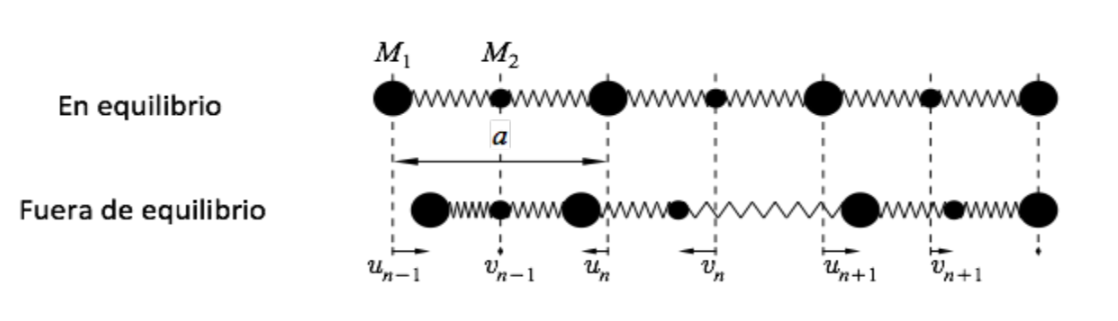
\includegraphics[width=0.9\textwidth]{cadena_diatomica.png}
     \label{fig:cadena}
  \end{figure}

  Considere como desplazamiento de los átomos de la n-ésima celda a

  \[
  M_{1}: \quad u_{n}(t)=u(k)e^{i(kna-\omega t)}
  \]
  \[
  M_{2}: \quad v_{n}(t)=v(k)e^{i(kna-\omega t)}
  \]

  \begin{enumerate}[label=\alph*)]
    \item Con ayuda de esquemas o dibujos haga un análisis de las fuerzas a primeros vecinos sobre el átomo de masa \( M_{1} \) y masa \( M_{2} \) y muestre que
    \[
    M_{1}\ddot{u}_{n}(t)=-\beta[2u_{n}-v_{n}-v_{n-1}]
    \]
    \[
    M_{2}\ddot{v}_{n}(t)=-\beta[2v_{n}-u_{n+1}-u_{n}]
    \]

    \item Sustituyendo las expresiones de los desplazamientos en las ecuaciones de movimiento, encuentre que:
    \[
    -\omega^{2}M_{1}u(k)=-2\beta u(k)+\beta v(k)(1+e^{-ika})
    \]
    \[
    -\omega^{2}M_{2}v(k)=-2\beta v(k)+\beta u(k)(1+e^{ika})
    \]

    \item La solución al sistema es la no trivial si el determinante de los coeficientes de las amplitudes es cero. Establezca que el determinante del sistema es
    \[
    \left|
    \begin{array}{cc}
    -\omega^{2}M_{1}+2\beta & -2\beta e^{-ika/2}\cos\!\left(\frac{1}{2}ka\right)\\[6pt]
    -2\beta e^{ika/2}\cos\!\left(\frac{1}{2}ka\right) & -\omega^{2}M_{2}+2\beta
    \end{array}
    \right|=0
    \]

    \item De la ecuación característica que resulta del inciso c), encuentre que la relación de dispersión es
    \[
    \omega^{2}_{\pm}(k)=\frac{\beta}{M_{1}M_{2}}\left\{(M_{1}+M_{2})\pm
    \sqrt{(M_{1}+M_{2})^{2}-4M_{1}M_{2}\sin^{2}\!\left(\frac{1}{2}ka\right)}\right\}
    \]

    \item Mostrar que cuando \( k=\pm\pi/a \) la razón entre las amplitudes de los desplazamientos de los átomos de masa \( M_{1} \) y masa \( M_{2} \) es cero o infinita, lo que implica que solo un tipo de átomo participa en la vibración.

    \item Mostrar que la velocidad de grupo es cero en los extremos de la primera zona de Brillouin, lo que indica ondas estacionarias.
  \end{enumerate}
\end{enumerate}
\end{AGbox}
\vspace{0.5cm}

\textcolor{Cinnabar}{\textbf{Solución:}}

\textbf{Inciso a)}\;

Para obtener las \textbf{ecuaciones de movimiento} con interacción a \emph{primeros vecinos}, 
analizamos la geometría de la cadena de la Fig.~\ref{fig:cadena_diatomica_2}, 
a partir de la cual fijamos la \textbf{celda unitaria} y la notación de índices

\begin{figure}[H]
  \centering
  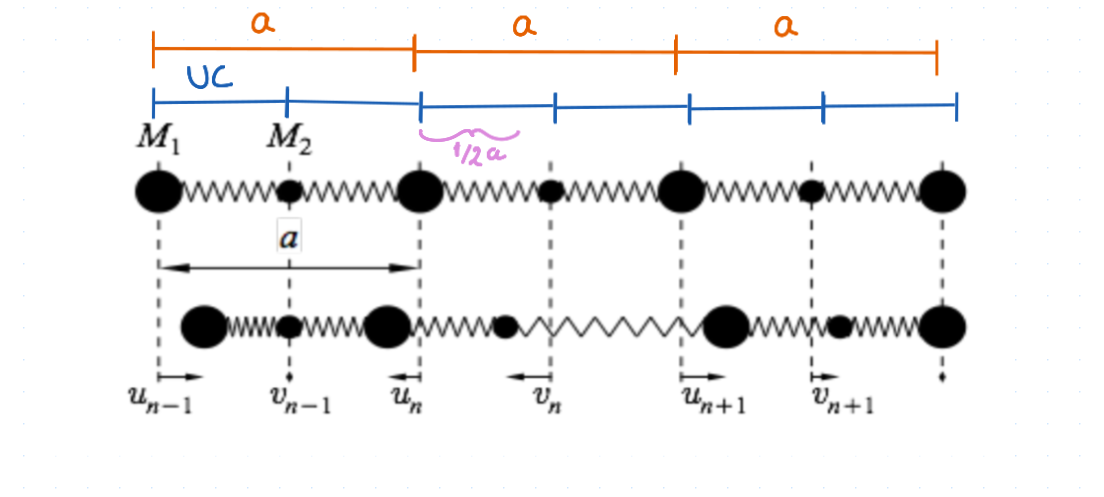
\includegraphics[width=0.93\textwidth]{cadena_diatomica_2.png}
  \caption{Cadena diatómica 1D con átomos alternados \(M_{1}\) y \(M_{2}\),
  acoplados mediante resortes idénticos de constante \(\beta\).
  La distancia de equilibrio entre átomos consecutivos es \(a/2\)}
  \label{fig:cadena_diatomica_2}
\end{figure}

Cada celda unitaria (\textcolor{trueblue}{\textbf{unit cell <<UC>>}}) contiene la pareja \((M_{1},M_{2})\) separada por \(a/2\) y las celdas se repiten con paso \(a\).
Numeramos las celdas con \(n\in\mathbb{Z}\).
En \textbf{equilibrio}, las posiciones de los átomos de la celda \(n\) son
\begin{equation}
\begin{split}
x_{n,0}^{(1)} &= n a,\\
x_{n,0}^{(2)} &= n a + \tfrac{a}{2}
\end{split}
\label{eq:pos_equilibrio}
\end{equation}
y, al perturbar el sistema, definimos desplazamientos longitudinales \(u_{n}(t)\) y \(v_{n}(t)\) tales que las
\textbf{posiciones instantáneas} quedan
\begin{equation}
\begin{split}
x_{n}^{(1)}(t) &= x_{n,0}^{(1)} + u_{n}(t) \;=\; n a + u_{n}(t),\\
x_{n}^{(2)}(t) &= x_{n,0}^{(2)} + v_{n}(t) \;=\; n a + \tfrac{a}{2} + v_{n}(t)
\end{split}
\label{eq:pos_instantaneas}
\end{equation}

Con esta convención, los \emph{primeros vecinos} de \(M_{1}(n)\) son \(M_{2}(n-1)\) y \(M_{2}(n)\); 
los de \(M_{2}(n)\) son \(M_{1}(n)\) y \(M_{1}(n+1)\)

\textcolor{trueblue}{\textbf{Ley de Hooke y elongación de un resorte.}}
La fuerza que ejerce un resorte de constante \(\beta\) es proporcional a su \emph{elongación} respecto a la longitud de equilibrio \(\ell_{0}=a/2\):
\begin{equation}
F \;=\; -\beta\,\Delta\ell, 
\qquad 
\Delta\ell \;=\; \text{(longitud actual)} - \ell_{0}
\label{eq:hooke}
\end{equation}
El signo negativo en \eqref{eq:hooke} indica que la fuerza es restauradora: se opone a la deformación del resorte

\textcolor{Tarawera}{\textbf{Fuerzas sobre la masa \(M_{1}(n)\).}}
Tomamos como positivas las fuerzas y desplazamientos hacia la derecha. Además de \eqref{eq:pos_instantaneas},
necesitaremos la posición del vecino \(M_{2}(n-1)\):
\begin{equation}
x_{n-1}^{(2)}(t) \;=\; (n-1)a + \tfrac{a}{2} + v_{n-1}(t) \;=\; n a - \tfrac{a}{2} + v_{n-1}(t)
\label{eq:pos_m2_n_1}
\end{equation}

\emph{Resorte derecho} \([\,M_{1}(n)\text{--}M_{2}(n)\,]\): su longitud actual es \(\ell_{R}=x_{n}^{(2)}-x_{n}^{(1)}\).
La \emph{elongación} y la fuerza sobre \(M_{1}(n)\) son
\begin{equation}
\begin{split}
\Delta\ell_{R}(t) 
&= \big[x_{n}^{(2)}(t)-x_{n}^{(1)}(t)\big]-\tfrac{a}{2} 
= \Big(n a + \tfrac{a}{2} + v_{n}\Big)-\Big(n a + u_{n}\Big)-\tfrac{a}{2} 
= v_{n}-u_{n}
\end{split}
\label{eq:elongacion_derecha}
\end{equation}
\begin{equation}
F_{R\to M_1} \;=\; -\,\beta\Big[x_{n}^{(1)}-x_{n}^{(2)}+\tfrac{a}{2}\Big]
\;=\; -\,\beta\,(u_{n}-v_{n})
\label{eq:fuerza_derecha}
\end{equation}

\emph{Resorte izquierdo} \([\,M_{2}(n-1)\text{--}M_{1}(n)\,]\): su longitud actual es \(\ell_{L}=x_{n}^{(1)}-x_{n-1}^{(2)}\).
La \emph{elongación} y la fuerza sobre \(M_{1}(n)\) son
\begin{equation}
\begin{split}
\Delta\ell_{L}(t) 
&= \big[x_{n}^{(1)}(t)-x_{n-1}^{(2)}(t)\big]-\tfrac{a}{2} 
= \Big(n a + u_{n}\Big)-\Big(n a - \tfrac{a}{2} + v_{n-1}\Big)-\tfrac{a}{2} 
= u_{n}-v_{n-1}
\end{split}
\label{eq:elongacion_izquierda}
\end{equation}
\begin{equation}
F_{L\to M_1} \;=\; -\,\beta\Big[x_{n}^{(1)}-x_{n-1}^{(2)}-\tfrac{a}{2}\Big]
\;=\; -\,\beta\,(u_{n}-v_{n-1})
\label{eq:fuerza_izquierda}
\end{equation}

Sumando \eqref{eq:fuerza_derecha} y \eqref{eq:fuerza_izquierda}, la \textbf{fuerza total} sobre \(M_{1}(n)\) es
\begin{equation}
\begin{split}
F_{M_{1}}(n) 
&= F_{L\to M_1} + F_{R\to M_1} 
= -\beta\,(u_{n}-v_{n-1}) - \beta\,(u_{n}-v_{n}) \\[2pt]
&= -\beta\Big[(u_{n}-v_{n}) + (u_{n}-v_{n-1})\Big]
\end{split}
\label{eq:F_M1}
\end{equation}

\textcolor{Tarawera}{\textbf{Fuerzas sobre la masa \(M_{2}(n)\).}}
Análogamente, \(M_{2}(n)\) se conecta con \(M_{1}(n)\) (izquierda) y \(M_{1}(n+1)\) (derecha).
Usando \(x_{n+1}^{(1)}(t)= (n+1)a + u_{n+1}(t)\), se obtiene
\begin{equation}
\begin{split}
\Delta\ell^{(M_2)}_{L} &= (x_{n}^{(1)}-x_{n}^{(2)})+\tfrac{a}{2} = (u_{n}-v_{n}),\\
\Delta\ell^{(M_2)}_{R} &= (x_{n+1}^{(1)}-x_{n}^{(2)})-\tfrac{a}{2} = (u_{n+1}-v_{n})
\end{split}
\label{eq:elongaciones_M2}
\end{equation}
y por \eqref{eq:hooke}, las fuerzas sobre \(M_{2}(n)\) son
\begin{equation}
\begin{split}
F^{(M_2)}_{L} &= -\beta\,(v_{n}-u_{n}),\\
F^{(M_2)}_{R} &= -\beta\,(v_{n}-u_{n+1})
\end{split}
\label{eq:fuerzas_M2}
\end{equation}
de modo que la \textbf{fuerza total} queda
\begin{equation}
F_{M_{2}}(n) \;=\; -\beta\Big[(v_{n}-u_{n}) + (v_{n}-u_{n+1})\Big]
\label{eq:F_M2}
\end{equation}

\textcolor{trueblue}{\textbf{Ecuaciones de movimiento.}}
Aplicando la segunda ley de Newton a \(M_{1}(n)\) y \(M_{2}(n)\), y sustituyendo \eqref{eq:F_M1} y \eqref{eq:F_M2}, resulta
\begin{equation}
\begin{split}
M_{1}\ddot{u}_{n}(t) &= F_{M_{1}}(n)\\
                     &= -\beta\big[2u_{n}-v_{n}-v_{n-1}\big]
\end{split}
\label{eq:mov_M1}
\end{equation}
\begin{equation}
\begin{split}
M_{2}\ddot{v}_{n}(t) &= F_{M_{2}}(n)\\
                     &= -\beta\big[2v_{n}-u_{n}-u_{n+1}\big]
\end{split}
\label{eq:mov_M2}
\end{equation}

Las expresiones \eqref{eq:mov_M1}–\eqref{eq:mov_M2} son exactamente las \textbf{ecuaciones de movimiento} pedidas para el inciso \textbf{a)}, 
y describen la dinámica longitudinal con interacción a primeros vecinos.

\fbox{\textbf{Inciso b)}}\;

Ahora sustituimos las expresiones de los \textbf{desplazamientos de los átomos} en las ecuaciones de movimiento \eqref{eq:mov_M1}–\eqref{eq:mov_M2}.  
Suponemos que cada átomo de la cadena oscila armónicamente, de modo que su desplazamiento tiene la forma:
\begin{equation}
\begin{split}
u_{n}(t) &= u(k)\,e^{\,i(kna-\omega t)}\\
v_{n}(t) &= v(k)\,e^{\,i(kna-\omega t)}
\end{split}
\label{eq:desplazamientos_b}
\end{equation}
donde \(u(k)\) y \(v(k)\) representan las \textbf{amplitudes de vibración} de los átomos \(M_{1}\) y \(M_{2}\), respectivamente.  
Estas amplitudes son constantes en el tiempo, mientras que toda la variación temporal y espacial está contenida en el factor exponencial \(e^{\,i(kna-\omega t)}\).

\vspace{0.4cm}
\textcolor{trueblue}{\textbf{Desplazamientos de los átomos vecinos.}}  
Los átomos que interactúan con \(M_{1}(n)\) y \(M_{2}(n)\) son sus \emph{primeros vecinos}.  
De \eqref{eq:desplazamientos_b} obtenemos directamente:
\begin{equation}
\begin{split}
v_{n-1}(t) &= v(k)\,e^{\,i[k(n-1)a-\omega t]} = v(k)\,e^{-ika}\,e^{\,i(kna-\omega t)}\\
u_{n+1}(t) &= u(k)\,e^{\,i[k(n+1)a-\omega t]} = u(k)\,e^{ika}\,e^{\,i(kna-\omega t)}
\end{split}
\label{eq:vecinos_b}
\end{equation}

\vspace{0.4cm}
\textcolor{trueblue}{\textbf{Derivadas temporales.}}  
Como las amplitudes \(u(k)\) y \(v(k)\) \emph{no dependen del tiempo}, al derivar con respecto a \(t\) sólo actúa el operador
\(\frac{d}{dt}\) sobre el factor exponencial \(e^{\,i(kna-\omega t)}\). Usemos explícitamente la \textbf{regla de la cadena}:

\begin{equation}
\frac{d}{dt}\Big(e^{\,i(kna-\omega t)}\Big)
= e^{\,i(kna-\omega t)}\;\frac{d}{dt}\big(i(kna-\omega t)\big)
= e^{\,i(kna-\omega t)}\;\big(i\cdot(-\omega)\big)
= -\,i\omega\,e^{\,i(kna-\omega t)}
\label{eq:derivada_exp}
\end{equation}

Aplicando \eqref{eq:derivada_exp} a cada desplazamiento:

\begin{equation}
\begin{split}
\dot{u}_{n}(t) 
&= \frac{d}{dt}\Big(u(k)\,e^{\,i(kna-\omega t)}\Big)
= u(k)\,\frac{d}{dt}\Big(e^{\,i(kna-\omega t)}\Big)\\[4pt]
&= u(k)\,\big(-\,i\omega\big)\,e^{\,i(kna-\omega t)}
= -\,i\omega\,u(k)\,e^{\,i(kna-\omega t)}
\end{split}
\label{eq:primera_u_ext}
\end{equation}

\begin{equation}
\begin{split}
\dot{v}_{n}(t) 
&= \frac{d}{dt}\Big(v(k)\,e^{\,i(kna-\omega t)}\Big)
= v(k)\,\frac{d}{dt}\Big(e^{\,i(kna-\omega t)}\Big)\\[4pt]
&= v(k)\,\big(-\,i\omega\big)\,e^{\,i(kna-\omega t)}
= -\,i\omega\,v(k)\,e^{\,i(kna-\omega t)}
\end{split}
\label{eq:primera_v_ext}
\end{equation}

\vspace{0.35cm}
Para las \textbf{segundas derivadas} (aceleraciones), derivamos de nuevo \eqref{eq:primera_u_ext}–\eqref{eq:primera_v_ext}.
Observa que \(-\,i\omega\) es una constante respecto a \(t\), así que vuelve a actuar \eqref{eq:derivada_exp} sobre el
exponencial:

\begin{equation}
\begin{split}
\ddot{u}_{n}(t) 
&= \frac{d}{dt}\Big(-\,i\omega\,u(k)\,e^{\,i(kna-\omega t)}\Big)
= -\,i\omega\,u(k)\,\frac{d}{dt}\Big(e^{\,i(kna-\omega t)}\Big)\\[4pt]
&= -\,i\omega\,u(k)\,\big(-\,i\omega\big)\,e^{\,i(kna-\omega t)}
= \underbrace{\big((-i)(-i)\big)}_{=-1}\,\omega^{2}\,u(k)\,e^{\,i(kna-\omega t)}\\[4pt]
&= -\,\omega^{2}\,u(k)\,e^{\,i(kna-\omega t)}
\end{split}
\label{eq:segunda_u_ext}
\end{equation}

\begin{equation}
\begin{split}
\ddot{v}_{n}(t) 
&= \frac{d}{dt}\Big(-\,i\omega\,v(k)\,e^{\,i(kna-\omega t)}\Big)
= -\,i\omega\,v(k)\,\frac{d}{dt}\Big(e^{\,i(kna-\omega t)}\Big)\\[4pt]
&= -\,i\omega\,v(k)\,\big(-\,i\omega\big)\,e^{\,i(kna-\omega t)}
= \big((-i)(-i)\big)\,\omega^{2}\,v(k)\,e^{\,i(kna-\omega t)}\\[4pt]
&= -\,\omega^{2}\,v(k)\,e^{\,i(kna-\omega t)}
\end{split}
\label{eq:segunda_v_ext}
\end{equation}

De \eqref{eq:segunda_u_ext}–\eqref{eq:segunda_v_ext} tenemos que las \textbf{aceleraciones} son:
\begin{equation}
\begin{split}
\ddot{u}_{n}(t) &= -\,\omega^{2}\,u(k)\,e^{\,i(kna-\omega t)}\\
\ddot{v}_{n}(t) &= -\,\omega^{2}\,v(k)\,e^{\,i(kna-\omega t)}
\end{split}
\label{eq:aceleraciones_b}
\end{equation}


\vspace{0.4cm}
\textcolor{trueblue}{\textbf{Sustitución en la ecuación de movimiento de \(M_{1}\).}}  
De \eqref{eq:mov_M1}:
\[
M_{1}\ddot{u}_{n}(t) = -\beta\,[\,2u_{n}(t)-v_{n}(t)-v_{n-1}(t)\,]
\]
Sustituyendo \eqref{eq:desplazamientos_b}, \eqref{eq:vecinos_b} y \eqref{eq:aceleraciones_b}:
\begin{equation}
\begin{split}
M_{1}\big(-\omega^{2}u(k)e^{\,i(kna-\omega t)}\big)
&= -\beta\Big[2u(k)e^{\,i(kna-\omega t)} - v(k)e^{\,i(kna-\omega t)} - v(k)e^{-ika}e^{\,i(kna-\omega t)}\Big]
\end{split}
\end{equation}
El factor \(e^{\,i(kna-\omega t)}\) está presente en todos los términos, por lo que se puede cancelar.  
Así se obtiene:
\begin{equation}
\begin{split}
-\omega^{2}M_{1}\,u(k)
&= -\beta\,[\,2u(k)-v(k)-v(k)e^{-ika}\,]\\
&= -2\beta\,u(k)+\beta\,v(k)\,[\,1+e^{-ika}\,]
\end{split}
\label{eq:ecuacion_M1_b}
\end{equation}

\vspace{0.4cm}
\textcolor{trueblue}{\textbf{Sustitución en la ecuación de movimiento de \(M_{2}\).}}  
De \eqref{eq:mov_M2}:
\[
M_{2}\ddot{v}_{n}(t) = -\beta\,[\,2v_{n}(t)-u_{n}(t)-u_{n+1}(t)\,]
\]
Sustituyendo las mismas expresiones:
\begin{equation}
\begin{split}
M_{2}\big(-\omega^{2}v(k)e^{\,i(kna-\omega t)}\big)
&= -\beta\Big[2v(k)e^{\,i(kna-\omega t)} - u(k)e^{\,i(kna-\omega t)} - u(k)e^{ika}e^{\,i(kna-\omega t)}\Big]
\end{split}
\end{equation}
Cancelando el factor común \(e^{\,i(kna-\omega t)}\), resulta:
\begin{equation}
\begin{split}
-\omega^{2}M_{2}\,v(k)
&= -\beta\,[\,2v(k)-u(k)-u(k)e^{ika}\,]\\
&= -2\beta\,v(k)+\beta\,u(k)\,[\,1+e^{ika}\,]
\end{split}
\label{eq:ecuacion_M2_b}
\end{equation}

\vspace{0.4cm}
Las ecuaciones \eqref{eq:ecuacion_M1_b}–\eqref{eq:ecuacion_M2_b} representan el \textbf{sistema algebraico} que relaciona las amplitudes \(u(k)\) y \(v(k)\) de los dos tipos de átomos para cada número de onda \(k\):
\[
\boxed{
\begin{aligned}
-\omega^{2}M_{1}\,u(k) &= -2\beta\,u(k)+\beta\,v(k)\,[\,1+e^{-ika}\,]\\
-\omega^{2}M_{2}\,v(k) &= -2\beta\,v(k)+\beta\,u(k)\,[\,1+e^{ika}\,]
\end{aligned}
}
\]


\fbox{\textbf{Inciso c)}}\;

A partir del sistema algebraico obtenido en el inciso b), \eqref{eq:ecuacion_M1_b}–\eqref{eq:ecuacion_M2_b}, reordenamos
los términos para escribirlo como un sistema lineal en las amplitudes \(u(k)\) y \(v(k)\):

\begin{equation}
\begin{split}
\big(-\omega^{2}M_{1}+2\beta\big)\,u(k)\;-\;\beta\big(1+e^{-ika}\big)\,v(k) \;=\; 0\\
-\beta\big(1+e^{ika}\big)\,u(k)\;+\;\big(-\omega^{2}M_{2}+2\beta\big)\,v(k) \;=\; 0
\end{split}
\label{eq:sistema_lineal_c}
\end{equation}

En forma matricial, el sistema que describe \eqref{eq:sistema_lineal_c} se puede escribir como:
\begin{equation}
\begin{pmatrix}
-\omega^{2}M_{1}+2\beta & -\beta\big(1+e^{-ika}\big)\\[4pt]
-\beta\big(1+e^{ika}\big) & -\omega^{2}M_{2}+2\beta
\end{pmatrix}
\begin{pmatrix}
u(k)\\[2pt] v(k)
\end{pmatrix}
=
\begin{pmatrix}
0\\[2pt] 0
\end{pmatrix}
\label{eq:matriz_cruda_c}
\end{equation}

Para que este sistema homogéneo tenga una solución no trivial \(\big(u(k),v(k)\big)\neq(0,0)\),
el \textbf{determinante} de la matriz de coeficientes debe anularse:
\begin{equation}
\det
\begin{pmatrix}
-\omega^{2}M_{1}+2\beta & -\beta\big(1+e^{-ika}\big)\\[4pt]
-\beta\big(1+e^{ika}\big) & -\omega^{2}M_{2}+2\beta
\end{pmatrix}
=0
\label{eq:cond_no_trivialidad}
\end{equation}

Los términos fuera de la \textbf{diagonal principal} del sistema matricial contienen los factores
\(\,1+e^{\pm ika}\,\), los cuales provienen de la suma de dos exponentes complejos.  
Estos factores aparecen con signo positivo o negativo en el exponente dependiendo de si el acoplamiento
considera un desplazamiento hacia la derecha (\(+ka\)) o hacia la izquierda (\(-ka\)).  

Para analizarlos con mayor claridad, es útil \textbf{separar la parte real y la parte compleja pura} del término
exponencial. Recordemos que un número complejo de la forma \(e^{i\theta}\) puede escribirse en su
representación trigonométrica como:
\[
e^{i\theta} = \cos\theta + i\sin\theta
\]
De modo que la suma \(1 + e^{i\theta}\) se convierte en:
\[
1 + e^{i\theta} = 1 + \cos\theta + i\sin\theta
\]
El primer término \(1+\cos\theta\) es real, mientras que \(i\sin\theta\) representa la componente imaginaria.  
Sin embargo, esta forma no es la más compacta ni la más conveniente para el análisis matricial, ya que
mezcla explícitamente las partes real e imaginaria.  
Tenemos:

% Demostración detallada de: 1 + e^{i\theta} = 2\,e^{i\theta/2}\cos(\theta/2)


\begin{equation}
\begin{split}
1 + e^{i\theta}
&= \underbrace{e^{i\theta/2}e^{-i\theta/2}}_{=\,1} \;+\; e^{i\theta}\\[4pt]
&= \underbrace{e^{i\theta/2}e^{-i\theta/2}}_{=\,1} \;+\; \underbrace{e^{i\theta/2}\,e^{i\theta/2}}_{=\,e^{i\theta}} \\[4pt]
&= e^{i\theta/2}\Big(\,e^{-i\theta/2} + e^{i\theta/2}\,\Big) \\[6pt]
&= e^{i\theta/2}\,\Big(2\cos(\tfrac{\theta}{2})\Big) \qquad \text{(pues $e^{ix}+e^{-ix}=2\cos x$)} \qquad \text{es decir} \qquad \boxed{(\cos x + i \sen x) + (\cos x - i \sen x)} \\[6pt]
&= 2\,e^{i\theta/2}\,\cos\!\Big(\tfrac{\theta}{2}\Big).
\end{split}
\label{eq:identidad_suma_exp_positiva}
\end{equation}


La igualdad anterior muestra que $1+e^{i\theta}$ es el producto de:
\begin{itemize}
  \item[$\bullet$] un \textbf{factor real} $2\cos(\theta/2)$
  \item[$\bullet$] y una \textbf{fase} $e^{i\theta/2}$
\end{itemize}

Aplicando estas identidades al caso de la cadena diatómica, donde \(\theta = ka\),
se obtiene finalmente:
\begin{equation}
1 + e^{\pm ika} = 2\,e^{\pm ika/2}\,\cos\!\Big(\tfrac{ka}{2}\Big)
\label{eq:identidad_suma_exp_final}
\end{equation}

Esta reescritura es fundamental, pues transforma la matriz compleja en una forma equivalente más simple
y simétrica, donde la parte relevante para el cálculo del determinante es completamente real.


Sustituyendo \eqref{eq:identidad_suma_exp_final} en los elementos fuera de la diagonal de \eqref{eq:matriz_cruda_c} se obtiene:
\begin{equation}
-\beta\big(1+e^{-ika}\big) \;=\; -2\beta\,e^{-ika/2}\cos\!\Big(\tfrac{ka}{2}\Big),
\qquad
-\beta\big(1+e^{ika}\big) \;=\; -2\beta\,e^{ika/2}\cos\!\Big(\tfrac{ka}{2}\Big)
\label{eq:acoplos_simplificados}
\end{equation}

Con esto, el sistema matricial adopta la forma simplificada:
\begin{equation}
\begin{pmatrix}
-\omega^{2}M_{1}+2\beta
& -2\beta\,e^{-ika/2}\cos\!\big(\tfrac{ka}{2}\big)\\[6pt]
-2\beta\,e^{ika/2}\cos\!\big(\tfrac{ka}{2}\big)
& -\omega^{2}M_{2}+2\beta
\end{pmatrix}
\begin{pmatrix}
u(k)\\[2pt] v(k)
\end{pmatrix}
=
\begin{pmatrix}
0\\[2pt] 0
\end{pmatrix}
\label{eq:matriz_simplificada_c}
\end{equation}



Finalmente, imponiendo la condición de no trivialidad \eqref{eq:cond_no_trivialidad} sobre la matriz ya simplificada \eqref{eq:matriz_simplificada_c}, se obtiene:
\begin{equation}
\left|
\begin{array}{cc}
-\omega^{2}M_{1}+2\beta & -2\beta\,e^{-ika/2}\cos\!\left(\tfrac{ka}{2}\right)\\[6pt]
-2\beta\,e^{ika/2}\cos\!\left(\tfrac{ka}{2}\right) & -\omega^{2}M_{2}+2\beta
\end{array}
\right| \;=\; 0
\label{eq:determinante_c}
\end{equation}


\fbox{\textbf{Inciso d)}}\;

A partir de la condición de no trivialidad \eqref{eq:determinante_c}, el determinante de la matriz debe anularse:
\begin{equation}
\Big(-\omega^{2}M_{1}+2\beta\Big)\Big(-\omega^{2}M_{2}+2\beta\Big)
-\Big(2\beta\cos\tfrac{ka}{2}\Big)^{2}=0
\label{eq:ecuacion_caracteristica_d}
\end{equation}

Desarrollamos el primer producto y dejamos indicado el cuadrado de los do términs  $\color{orange(colorwheel)}\boldsymbol{-2\beta\,e^{-ika/2}\cos\!\left(\tfrac{ka}{2}\right)}$ :
\begin{equation}
\begin{split}
\Big(-\omega^{2}M_{1}+2\beta\Big)\Big(-\omega^{2}M_{2}+2\beta\Big)
&=\;(+\,\omega^{4}M_{1}M_{2})
+(-\,2\beta\,\omega^{2}M_{1})\\
&\quad +(-\,2\beta\,\omega^{2}M_{2})
+(4\beta^{2})
\end{split}
\label{eq:producto_d}
\end{equation}

Sustituyendo \eqref{eq:producto_d} en \eqref{eq:ecuacion_caracteristica_d} y agrupando en potencias de \(\omega\):
\begin{equation}
\omega^{4}M_{1}M_{2}-2\beta(M_{1}+M_{2})\,\omega^{2}
+4\beta^{2}-\Big(2\beta\cos\tfrac{ka}{2}\Big)^{2}=0
\label{eq:previo_trig_d}
\end{equation}

Aplicamos la identidad trigonométrica \(\boxed{\cos^{2}x=1-\sin^{2}x}\) al último término de \eqref{eq:previo_trig_d}, tenemos:
\begin{equation}
\Big(2\beta\cos\tfrac{ka}{2}\Big)^{2}
=4\beta^{2}\cos^{2}\tfrac{ka}{2}
=4\beta^{2}\Big(1-\sin^{2}\tfrac{ka}{2}\Big)
\label{eq:expansion_trig_d}
\end{equation}

Sustituyendo \eqref{eq:expansion_trig_d} en \eqref{eq:previo_trig_d} se cancelan los términos constantes \(4\beta^{2}\) y queda:
\begin{equation}
M_{1}M_{2}\,\omega^{4}-2\beta(M_{1}+M_{2})\,\omega^{2}
+4\beta^{2}\sin^{2}\!\Big(\tfrac{ka}{2}\Big)=0
\label{eq:ecuacion_cuadratica_d}
\end{equation}

Sea \(X\equiv\omega^{2}\). La \eqref{eq:ecuacion_cuadratica_d} es cuadrática en \(X\) con
\[
A=M_{1}M_{2},\qquad B=-2\beta(M_{1}+M_{2}),\qquad
C=4\beta^{2}\sin^{2}\!\Big(\tfrac{ka}{2}\Big)
\]
Aplicamos la fórmula general (\textbf{ec. de  Bhaskara}) \(AX^{2}+BX+C=0\Rightarrow
X=\dfrac{-B\pm\sqrt{B^{2}-4AC}}{2A}\):

\begin{equation}
\omega^{2}=\frac{2\beta(M_{1}+M_{2})\;\pm\;
\sqrt{\;\big[-2\beta(M_{1}+M_{2})\big]^{2}
-4(M_{1}M_{2})\big[4\beta^{2}\sin^{2}(\tfrac{ka}{2})\big]\;}}{2M_{1}M_{2}}
\label{eq:aplicacion_formula_general_d}
\end{equation}

Simplificamos el radicando extrayendo el factor común \(4\beta^{2}\):
\begin{equation}
\sqrt{\,4\beta^{2}\Big[(M_{1}+M_{2})^{2}-4M_{1}M_{2}\sin^{2}\!\Big(\tfrac{ka}{2}\Big)\Big]\,}
=2\beta\sqrt{(M_{1}+M_{2})^{2}-4M_{1}M_{2}\sin^{2}\!\Big(\tfrac{ka}{2}\Big)}
\label{eq:radicando_simplificado_d}
\end{equation}

Sustituyendo \eqref{eq:radicando_simplificado_d} en \eqref{eq:aplicacion_formula_general_d} y dividiendo numerador y denominador entre \(2M_{1}M_{2}\) obtenemos las dos ramas de la dispersión:
\begin{equation}
\boxed{\
\omega^{2}_{\pm}(k)=\frac{\beta}{M_{1}M_{2}}
\left[(M_{1}+M_{2})\pm
\sqrt{(M_{1}+M_{2})^{2}-4M_{1}M_{2}\sin^{2}\!\Big(\tfrac{ka}{2}\Big)}\right]
}
\label{eq:dispersion_d}
\end{equation}

\noindent
La solución con el signo “\(-\)” define la rama \emph{acústica} y la solución con el signo “\(+\)” la rama \emph{óptica}

% =======================
% Inciso e)
% =======================
% =======================
% Inciso e) – Versión extendida
% =======================
\fbox{\textbf{Inciso e)}}\;

\textcolor{Sun}{\textbf{Meta.}} Tenemos que demostrar que en el borde de la primera zona de Brillouin,
\textcolor{vividviolet}{\textbf{\(k=\pm\pi/a\)}}, la razón de amplitudes entre los desplazamientos de las masas \(M_{1}\) y \(M_{2}\) es
cero o infinita; es decir, en cada una de las dos soluciones sólo \underline{vibra \emph{un} tipo de átomo}.

Partimos del sistema obtenido en el inciso b), \eqref{eq:ecuacion_M1_b}–\eqref{eq:ecuacion_M2_b}:
\begin{equation}
\begin{split}
-\omega^{2}M_{1}\,u(k) &= -2\beta\,u(k)+\beta\,v(k)\,[\,1+e^{-ika}\,],\\
-\omega^{2}M_{2}\,v(k) &= -2\beta\,v(k)+\beta\,u(k)\,[\,1+e^{ika}\,]
\end{split}
\label{eq:e_sistema_partida}
\end{equation}

Cuando \textcolor{vividviolet}{\textbf{\(k=\pm\pi/a\)}}
En el borde de zona tenemos:
\[
e^{\pm ika}=e^{\pm i\pi}=-1
\quad\Rightarrow\quad
1+e^{\pm ika}=0.
\]
Sustituyendo en \eqref{eq:e_sistema_partida} se obtiene el siguiente sistema de ecuaciones homogéneo:
\begin{equation}
\begin{split}
\big(-\omega^{2}M_{1}+2\beta\big)\,u(k) &= 0,\\
\big(-\omega^{2}M_{2}+2\beta\big)\,v(k) &= 0
\end{split}
\label{eq:e_desacoplado}
\end{equation}

De \eqref{eq:e_desacoplado} se desprenden los dos \emph{casos individuales para las partículas}:

 \textbf{Caso A (modo de \(M_{1}\)).}
Suponiendo \(u(k)\neq 0\), la primera ecuación impone:
\begin{equation}
-\omega^{2}M_{1}+2\beta = 0
\quad\Rightarrow\quad
\boxed{\omega^{2}=\frac{2\beta}{M_{1}}}
\label{eq:e_omegaA}
\end{equation}

Sustituyendo este valor en la segunda ecuación del sistema original \eqref{eq:e_sistema_partida}, y recordando que \(1+e^{ika}=0\):
\begin{equation}
\big(-\omega^{2}M_{2}+2\beta\big)\,v(k) = 0
\label{eq:e_vk_reducida}
\end{equation}

Reemplazando ahora \(\omega^{2}=\frac{2\beta}{M_{1}}\) en \eqref{eq:e_vk_reducida}:
\begin{equation}
\begin{split}
\Big(-\frac{2\beta}{M_{1}}M_{2}+2\beta\Big)v(k) &= 0,\\[4pt]
2\beta\left(1-\frac{M_{2}}{M_{1}}\right)v(k) &= 0
\end{split}
\label{eq:e_vk_desarrollo}
\end{equation}

De \eqref{eq:e_vk_desarrollo}, si \(M_{1}=M_{2}\), el factor entre paréntesis se anula.  
Pero si \(M_{1}\neq M_{2}\), entonces:
\[
1-\frac{M_{2}}{M_{1}}\neq 0 \quad\Rightarrow\quad v(k)=0
\]
Por tanto:
\begin{equation}
\boxed{\;\dfrac{u(k)}{v(k)}\;\longrightarrow\;\infty\;}
\qquad\text{(sólo vibra la subred \(M_{1}\), a frecuencia \(\omega^{2}=2\beta/M_{1}\))}
\label{eq:e_razon_infinita}
\end{equation}

\textbf{Caso B (modo de \(M_{2}\)).}
Suponiendo \(v(k)\neq 0\), la segunda ecuación impone:
\begin{equation}
-\omega^{2}M_{2}+2\beta = 0
\quad\Rightarrow\quad
\boxed{\omega^{2}=\frac{2\beta}{M_{2}}}
\label{eq:e_omegaB}
\end{equation}

Sustituyendo este valor en la primera ecuación de \eqref{eq:e_sistema_partida} y usando \(1+e^{-ika}=0\):
\begin{equation}
\big(-\omega^{2}M_{1}+2\beta\big)\,u(k) = 0
\label{eq:e_uk_reducida}
\end{equation}

Reemplazamos \(\omega^{2}=\frac{2\beta}{M_{2}}\):
\begin{equation}
\begin{split}
\Big(-\frac{2\beta}{M_{2}}M_{1}+2\beta\Big)u(k) &= 0,\\[4pt]
2\beta\left(1-\frac{M_{1}}{M_{2}}\right)u(k) &= 0
\end{split}
\label{eq:e_uk_desarrollo}
\end{equation}

De \eqref{eq:e_uk_desarrollo}, para \(M_{1}\neq M_{2}\):
\[
1-\frac{M_{1}}{M_{2}}\neq 0 \quad\Rightarrow\quad u(k)=0
\]

Así:
\begin{equation}
\boxed{\;\dfrac{u(k)}{v(k)}\;=\;0\;}
\qquad\text{(sólo vibra la subred \(M_{2}\), a frecuencia \(\omega^{2}=2\beta/M_{2}\))}
\label{eq:e_razon_cero}
\end{equation}

La relación de dispersión hallada en \eqref{eq:dispersion_d} fue:
\[
\omega^{2}_{\pm}(k)=\frac{\beta}{M_{1}M_{2}}
\left[(M_{1}+M_{2})\pm\sqrt{(M_{1}+M_{2})^{2}-4M_{1}M_{2}\sin^{2}\!\Big(\tfrac{ka}{2}\Big)}\right]
\]
En \(k=\pm\pi/a\) se tiene \(\sin^{2}\!\big(\tfrac{ka}{2}\big)=1\), por lo que:
\[
\sqrt{(M_{1}+M_{2})^{2}-4M_{1}M_{2}}=\lvert M_{1}-M_{2}\rvert,
\]
y entonces:
\begin{equation}
\omega^{2}_{\pm}\Big(\tfrac{\pi}{a}\Big)=\frac{\beta}{M_{1}M_{2}}
\Big[(M_{1}+M_{2})\pm\lvert M_{1}-M_{2}\rvert\Big]
=\begin{cases}
\displaystyle \frac{2\beta}{M_{2}},\\[6pt]
\displaystyle \frac{2\beta}{M_{1}}
\end{cases}
\label{eq:e_match_dispersion}
\end{equation}

Es decir, las mismas frecuencias obtenidas en los casos anteriores.  
Si \(M_{1}>M_{2}\), entonces \(\omega^{2}_{+}=2\beta/M_{2}\) (modo óptico, alta frecuencia)
y \(\omega^{2}_{-}=2\beta/M_{1}\) (modo acústico, baja frecuencia).

A partir de la primera ecuación de \eqref{eq:e_sistema_partida}, puede escribirse la razón:
\[
\frac{u(k)}{v(k)}=\frac{\beta[1+e^{-ika}]}{\omega^{2}M_{1}-2\beta}
\]
Para \(k=\pi/a\), el numerador se anula \((1+e^{-ika}=0)\), por lo que:
\begin{itemize}
  \item[$\bullet$] Si \(\omega^{2}\neq 2\beta/M_{1}\), entonces \(\frac{u}{v}=0\Rightarrow\) modo indiividual de \(M_{2}\).
  \item[$\bullet$] Si \(\omega^{2}=2\beta/M_{1}\), el denominador se anula y \(\frac{u}{v}\to\infty\Rightarrow\) modo individual de \(M_{1}\).
\end{itemize}

Para \(k=\pi/a\), el factor espacial es:
\[
e^{ikna}=e^{i\pi n}=(-1)^{n}
\]
Por tanto:
\begin{equation}
u_{n}(t)=u\,(-1)^{n}e^{-i\omega t},\qquad
v_{n}(t)=v\,(-1)^{n}e^{-i\omega t}.
\label{eq:e_patron_espacial}
\end{equation}
De acuerdo con \eqref{eq:e_razon_infinita}–\eqref{eq:e_razon_cero}:
\begin{itemize}
  \item[$\bullet$] En el \textbf{modo imdividual de \(M_{1}\)} (\(v=0\)), sólo los \(M_{1}\) oscilan alternando signo entre celdas: \(+\,-\,+\,-\,\dots\)
  \item[$\bullet$] En el \textbf{modo individual de \(M_{2}\)} (\(u=0\)), sólo los \(M_{2}\) oscilan alternadamente con nodos en los \(M_{1}\)
\end{itemize}

En el borde de zona el acoplamiento entre celdas vecinas se anula \((1+e^{\pm i\pi}=0)\),
y cada subred vibra como un oscilador independiente:
\[
\omega^{2}=\frac{2\beta}{M_{1}} \quad\text{o}\quad \omega^{2}=\frac{2\beta}{M_{2}}.
\]
La subred más ligera oscila con frecuencia mayor (modo óptico),  
mientras que la más pesada lo hace con frecuencia menor (modo acústico).

En \(k=\pm\pi/a\) se cumple:
\[
\boxed{\;\dfrac{u(k)}{v(k)}\in\{\,0,\ \infty\,\}\;}
\]
y las únicas soluciones físicas son modos individuales de una u otra subred, con frecuencias
\(\omega^{2}=2\beta/M_{1}\) y \(\omega^{2}=2\beta/M_{2}\), en completo acuerdo con la relación de dispersión.


\fbox{\textbf{Inciso f)}}\;

\textcolor{trueblue}{\textbf{Enunciado.}} Mostrar que la \emph{velocidad de grupo}
\[
v_g(k)\;\equiv\;\frac{\mathrm d\omega}{\mathrm dk}
\]
se anula en los extremos de la primera zona de Brillouin, es decir, en
\(k=0\) (centro de zona) y \(k=\pm\pi/a\) (borde de zona). Esto implica
ondas estacionarias en esos puntos.

\vspace{0.4cm}
Del \textbf{inciso d)} (ec.~\eqref{eq:dispersion_d}), para las dos ramas \(\omega_\pm(k)\) se tiene:
\begin{equation}
\omega^{2}_{\pm}(k)
= \frac{\beta}{M_{1}M_{2}}\left[(M_{1}+M_{2})
\pm \sqrt{(M_{1}+M_{2})^{2}-4M_{1}M_{2}\sin^{2}\!\Big(\tfrac{ka}{2}\Big)}\right].
\label{eq:f_dispersion}
\end{equation}
Definamos a las siguientes variables:
\[q\equiv \frac{ka}{2},\qquad
\Delta(k)\equiv (M_{1}+M_{2})^{2}-4M_{1}M_{2}\sin^{2}q
\]

\vspace{0.4cm}
\textcolor{Tarawera}{\textbf{ Derivamos \(\omega(k)\) con respecto a \(k\).}}
Usamos que
\[
2\omega\,\frac{\mathrm d\omega}{\mathrm dk}
= \frac{\mathrm d}{\mathrm dk}\!\big(\omega^2\big)
\]
Derivando \eqref{eq:f_dispersion}:
\begin{equation}
\frac{\mathrm d}{\mathrm dk}\big(\omega_\pm^2\big)
= \frac{\beta}{M_1M_2}\left[
\pm \frac{1}{2\sqrt{\Delta(k)}}\,\frac{\mathrm d\Delta}{\mathrm dk}
\right].
\label{eq:f_domegacuad_dk}
\end{equation}
Como
\[
\frac{\mathrm d}{\mathrm dk}\sin^{2}q
= 2\sin q\cos q\,\frac{\mathrm dq}{\mathrm dk}
= \sin(2q)\,\frac{a}{2}
= \sin(ka)\,\frac{a}{2},
\]
se obtiene
\begin{equation}
\frac{\mathrm d\Delta}{\mathrm dk}
= -4M_1M_2\,\frac{\mathrm d}{\mathrm dk}\big(\sin^{2}q\big)
= -4M_1M_2\left(\frac{a}{2}\sin ka\right)
= -2a\,M_1M_2\,\sin(ka)
\label{eq:f_dDelta_dk}
\end{equation}
Sustituyendo \eqref{eq:f_dDelta_dk} en \eqref{eq:f_domegacuad_dk} y dividiendo por \(2\omega_\pm\):
\begin{equation}
v_g^{(\pm)}(k)\;=\;\frac{\mathrm d\omega_\pm}{\mathrm dk}
=\frac{1}{2\omega_\pm}\,\frac{\mathrm d(\omega_\pm^2)}{\mathrm dk}
= \mp\,\frac{\beta}{\omega_\pm(k)}\,
\frac{a}{2}\,\frac{\sin(ka)}{\sqrt{\Delta(k)}}
\label{eq:f_vg_general}
\end{equation}

\vspace{0.4cm}
\textcolor{Tarawera}{\textbf{Evaluamos en los extremos de la zona de Brillouin.}}
\begin{itemize}
  \item[$\bullet$] \(\boldsymbol{k=0}\): \(\sin(ka)=\sin 0=0\). De \eqref{eq:f_vg_general},
  \[
  v_g^{(\pm)}(0)=0
  \]
  \item[$\bullet$] \(\boldsymbol{k=\pm\pi/a}\) (frontera de zona): \(\sin(ka)=\sin(\pm\pi)=0\). De nuevo,
  \[
  v_g^{(\pm)}(\pm\pi/a)=0
  \]
\end{itemize}
En ambos extremos la \(\sin(ka)\) anula el numerador de \eqref{eq:f_vg_general}, mientras que
\(\omega_\pm\) y \(\sqrt{\Delta}\) son finitos y distintos de cero (salvo el caso
donde\(M_1=M_2\), que no altera el rsultado de \(v_g=0\))

\vspace{0.4cm}
La velocidad de grupo \(v_g\) mide la velocidad de transporte de energía/paquetes de onda.
Que \(v_g=0\) en \(k=0\) y \(k=\pm\pi/a\) significa que esos puntos son \emph{extremos}
(de hecho, máximos/mínimos) de \(\omega(k)\) para cada rama; allí las excitaciones forman
\textbf{ondas estacionarias}:
\begin{itemize}
  \item[$\bullet$] En \(k=0\): todos los átomos oscilan en fase (modo acústico) o fuera de fase entre subredes (modo óptico),
        pero sin transporte neto.
  \item\item[$\bullet$] En \(k=\pm\pi/a\): la fase espacial alterna \(+\,-\,+\,-\,\dots\) entre celdas (longitud de onda \(2a\));
        el acoplamiento entre celdas vecinas se cancela y cada subred vibra “localmente”, como se mostró en el inciso e).
\end{itemize}
\vspace{0.5cm}

\begin{AGbox}[8]
\begin{enumerate}[label={{\textcolor{trueblue}{\textbf{Pr.} \arabic*.2}}}, start=2]
  \item Considere una muestra cristalina cúbica simple cuyos átomos tienen masa $m$ y $\beta$ como la constante del resorte que representa la interacción con los primeros vecinos.
  
  

  \begin{figure}[H]
    \centering
    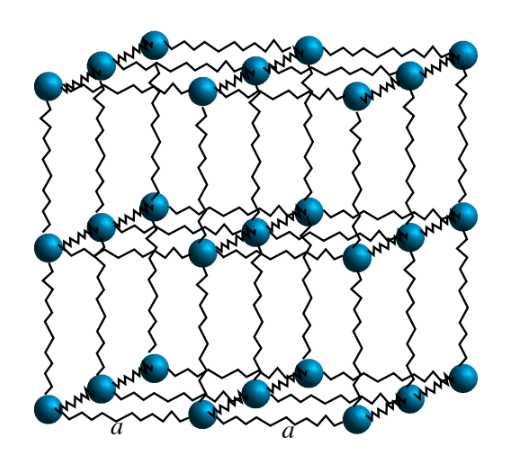
\includegraphics[width=0.4\textwidth]{red_cubica_simple.png}
    \label{fig:red_cubica}
  \end{figure}

  \begin{enumerate}[label=\alph*)]
    \item Tomando en cuenta sólo interacción a primeros vecinos, escriba la \textbf{fuerza total} sobre el átomo en la posición $\vec{r} = i a \hat{x} + j a \hat{y} + k a \hat{z}$.
    
    \item Halle la ecuación vectorial de movimiento del átomo del inciso a). Para ello, use la segunda ley de Newton y desplazamientos vectoriales del tipo
    \[
    \vec{u}(\vec{r},t) = \vec{u}(\vec{k})\exp\{i(\vec{k}\cdot\vec{r}-\omega t)\},
    \]
    donde $\vec{u}(\vec{k})$ es la amplitud vectorial de los desplazamientos con componentes
    \[
    \vec{u}(\vec{k}) = u_{x}\hat{x} + u_{y}\hat{y} + u_{z}\hat{z}.
    \]
    
    \item Del sistema de ecuaciones (una para cada dirección de movimiento del inciso b), deduzca los elementos de la matriz dinámica $\mathbf{D}$.
    \[
    \mathbf{D}=
    \begin{pmatrix}
    D_{xx} & D_{xy} & D_{xz}\\
    D_{yx} & D_{yy} & D_{yz}\\
    D_{zx} & D_{zy} & D_{zz}
    \end{pmatrix},
    \quad \text{tal que } \mathbf{D}\vec{u}=M\omega^{2}\vec{u}.
    \tag{1}
    \]
    
    \item Suponga el caso particular de una oscilación de la red que se propaga en dirección $\vec{k}=k_{x}\hat{x}+k_{y}\hat{y}+k_{z}\hat{z}=k\hat{x}+k\hat{y}$. Resuelva la ecuación (1) para hallar los valores de las frecuencias (eigen valores) en términos de $k$, es decir, halle la relación de dispersión.
    
    \item Haga un bosquejo de la relación de dispersión, $\omega(\vec{k})$, para “el recorrido” de valores $k$ 
    \[
    \Sigma (\text{sigma}) \rightarrow \Gamma (\text{gama}) \rightarrow \Delta (\text{delta}) \rightarrow X.
    \]
    
    \item Encuentre los eigen vectores de las frecuencias encontradas en el inciso d) e indique cuál corresponde al modo longitudinal y cuáles a los transversales.
  \end{enumerate}
\end{enumerate}
\end{AGbox}
\vspace{0.5cm}

\textcolor{Cinnabar}{\textbf{Solución:}}
\textbf{Inciso a)}\;

Imaginemos la red \textbf{cúbica simple} como un andamio 3D donde cada átomo está en una esquina del cubo de lado \(a\). El átomo que nos interesa está en
\[
\vec R = i\,a\,\hat x + j\,a\,\hat y + k\,a\,\hat z
\]
y sus \emph{primeros vecinos} son seis: uno a cada lado sobre los ejes \(x\), \(y\) y \(z\), todos a distancia \(a\). Es decir, están en \(\vec R \pm a\hat x\), \(\vec R \pm a\hat y\) y \(\vec R \pm a\hat z\)

Cada enlace con un vecino se comporta como un resorte con constante \(\beta\). Si el átomo en \(\vec R\) y su vecino se mueven un poco respecto al equilibrio, el resorte se estira o se comprime, y por la ley de Hooke aparece una fuerza restauradora. Para no enredarnos: sobre el enlace alineado con \(x\) sólo importa cuánto cambió la \emph{componente en \(x\)} del desplazamiento entre los dos átomos; lo mismo para \(y\) y para \(z\)

Denotemos el desplazamiento del átomo en \(\vec R\) como
\[
\vec u(\vec R,t)=u_x(\vec R,t)\,\hat x + u_y(\vec R,t)\,\hat y + u_z(\vec R,t)\,\hat z
\]
y consideremos primero el par de vecinos en la dirección \(x\). La variación de longitud efectiva del resorte de la derecha (\(+x\)) es la diferencia de las componentes en \(x\):
\[
\Delta\ell_{+x} = u_x(\vec R{+}a\hat x,t) - u_x(\vec R,t)
\]
y análogamente, para el resorte de la izquierda (\(-x\)):
\[
\Delta\ell_{-x} = u_x(\vec R{-}a\hat x,t) - u_x(\vec R,t)
\]
La fuerza que cada resorte ejerce sobre el átomo en \(\vec R\) apunta a lo largo del eje del resorte y es proporcional a \(-\Delta\ell\). Sumando las dos aportaciones sobre \(x\) queda
\[
F_x(\vec R,t)= -\beta\,\Delta\ell_{+x} \;-\; \beta\,\Delta\ell_{-x}
= \beta\Big[u_x(\vec R{+}a\hat x,t) + u_x(\vec R{-}a\hat x,t) - 2\,u_x(\vec R,t)\Big]
\]
Haciendo lo mismo en \(y\) y en \(z\), la \textbf{fuerza total} sobre el átomo en \(\vec R\) se obtiene componente a componente como
\begin{equation}
\boxed{
\begin{aligned}
F_x(\vec R,t)&=\beta\Big[u_x(\vec R{+}a\hat x,t)+u_x(\vec R{-}a\hat x,t)-2u_x(\vec R,t)\Big]\\
F_y(\vec R,t)&=\beta\Big[u_y(\vec R{+}a\hat y,t)+u_y(\vec R{-}a\hat y,t)-2u_y(\vec R,t)\Big]\\
F_z(\vec R,t)&=\beta\Big[u_z(\vec R{+}a\hat z,t)+u_z(\vec R{-}a\hat z,t)-2u_z(\vec R,t)\Big]
\end{aligned}}
\label{eq:fuerza_componentes_rcs}
\end{equation}

\fbox{\textbf{Inciso b)}}\;

Usamos ahora la segunda ley de Newton \(m\,\ddot{\vec u} = \vec F\) junto con la forma de onda propuesta para los desplazamientos del átomo:
\begin{equation}
\boxed{
\vec u(\vec r,t)=\vec u(\vec k)\,e^{\,i(\vec k\cdot\vec r-\omega t)}, \qquad 
\vec u(\vec k)=u_x\hat x+u_y\hat y+u_z\hat z
}
\label{eq:forma_onda}
\end{equation}

La aceleración temporal se obtiene derivando dos veces respecto al tiempo:
\begin{equation}
\ddot{\vec u}(\vec r,t) = -\,\omega^2\,\vec u(\vec k)\,e^{\,i(\vec k\cdot\vec r-\omega t)}
\label{eq:aceleracion}
\end{equation}

La estrategia está en cómo escribimos los desplazamientos de los vecinos.  
Por ejemplo, los que están a una distancia \(a\) sobre el eje \(x\) se expresan como:
\begin{equation}
u_x(\vec r{\pm}a\hat x,t)
= u_x(\vec k)\,e^{\,i(\vec k\cdot(\vec r{\pm}a\hat x)-\omega t)}
= u_x(\vec k)\,e^{\,i(\vec k\cdot\vec r-\omega t)}\,e^{\,\pm i k_x a}
\label{eq:desplazamientos_vecinos}
\end{equation}
y análogamente para los ejes \(y\) y \(z\)

Sustituimos \eqref{eq:forma_onda}, \eqref{eq:aceleracion} y \eqref{eq:desplazamientos_vecinos} en la expresión de la fuerza \eqref{eq:fuerza_componentes_rcs}.  
Para la dirección \(x\) tenemos:
\begin{equation}
\begin{split}
m\ddot u_x(\vec r,t)
&=F_x(\vec r,t)\\
-\,m\omega^2\,u_x(\vec k)\,e^{\,i(\vec k\cdot\vec r-\omega t)}
&=\beta\,u_x(\vec k)\,e^{\,i(\vec k\cdot\vec r-\omega t)}\big(e^{\,i k_x a}+e^{-i k_x a}-2\big)
\end{split}
\label{eq:newton_x}
\end{equation}

El factor exponencial \(e^{\,i(\vec k\cdot\vec r-\omega t)}\) aparece en ambos lados y puede eliminarse, quedando:
\begin{equation}
-\,m\omega^2\,u_x=\beta\big(e^{\,i k_x a}+e^{-i k_x a}-2\big)\,u_x
\label{eq:ecuacion_x_intermedia}
\end{equation}

Usando la identidad \(e^{ix}+e^{-ix}=2\cos x\) que hemos usado con anterioridad en la ecuación \eqref{eq:identidad_suma_exp_positiva}  y multiplicando ambos lados de la ec. \eqref{eq:ecuacion_x_intermedia} por el término $-1/m$ se simplifica a:
\begin{equation}
\omega^2\,u_x=\frac{2\beta}{m}\big(2-2\cos k_x a\big)\,u_x
=\frac{4\beta}{m}\sin^2\!\Big(\frac{k_x a}{2}\Big)u_x
\label{eq:ecuacion_x_final}
\end{equation}

El mismo procedimiento se aplica a las otras dos direcciones, obteniendo tres ecuaciones del mismo tipo:
\begin{equation}
\boxed{
\begin{aligned}
\omega^2\,u_x&=\tfrac{4\beta}{m}\sin^2\!\Big(\tfrac{k_x a}{2}\Big)u_x\\[4pt]
\omega^2\,u_y&=\tfrac{4\beta}{m}\sin^2\!\Big(\tfrac{k_y a}{2}\Big)u_y\\[4pt]
\omega^2\,u_z&=\tfrac{4\beta}{m}\sin^2\!\Big(\tfrac{k_z a}{2}\Big)u_z
\end{aligned}}
\label{eq:ecuaciones_cartesianas}
\end{equation}

Cada una corresponde a un modo de vibración independiente a lo largo de \(x\), \(y\) o \(z\).  
Las tres ecuaciones representan la \textbf{ecuación vectorial de movimiento} del átomo en la red cúbica simple bajo la suposición de ondas planas.  
Podemos reunirlas en una sola expresión compacta:
\begin{equation}
\boxed{
m\omega^2
\begin{pmatrix}
u_x\\u_y\\u_z
\end{pmatrix}
=
4\beta
\begin{pmatrix}
\sin^2(\tfrac{k_x a}{2})&0&0\\[4pt]
0&\sin^2(\tfrac{k_y a}{2})&0\\[4pt]
0&0&\sin^2(\tfrac{k_z a}{2})
\end{pmatrix}
\begin{pmatrix}
u_x\\u_y\\u_z
\end{pmatrix}
}
\label{eq:ecuacion_vectorial_movimiento}
\end{equation}


\fbox{\textbf{Inciso c)}}\;

La idea es tomar las tres ecuaciones del inciso b), escribirlas con el desplazamiento tipo onda
\(\vec u(\vec r,t)=\vec u(\vec k)\,e^{i(\vec k\cdot\vec r-\omega t)}\) y, de ahí, interpretar a la matriz dinámica \(\mathbf D\) tal que \(\mathbf D\,\vec u=m\omega^2\vec u\)

\medskip
Partimos de la fuerza total sobre el átomo en \(\vec R\), componente a componente, obtenida en el inciso a):
\begin{equation}
\boxed{
\begin{aligned}
F_x(\vec R,t)&=\beta\Big[u_x(\vec R{+}a\hat x,t)+u_x(\vec R{-}a\hat x,t)-2u_x(\vec R,t)\Big]\\
F_y(\vec R,t)&=\beta\Big[u_y(\vec R{+}a\hat y,t)+u_y(\vec R{-}a\hat y,t)-2u_y(\vec R,t)\Big]\\
F_z(\vec R,t)&=\beta\Big[u_z(\vec R{+}a\hat z,t)+u_z(\vec R{-}a\hat z,t)-2u_z(\vec R,t)\Big]
\end{aligned}}
\label{eq:c_fuerza_total}
\end{equation}

Aplicamos la segunda ley de Newton en cada eje:
\begin{equation}
m\,\ddot u_\alpha(\vec R,t)=F_\alpha(\vec R,t)\qquad(\alpha=x,y,z)
\label{eq:c_newton}
\end{equation}

Usamos ahora el desplazamiento tipo onda. Para \(\alpha=x\), escribimos
\begin{equation}
u_x(\vec R,t)=u_x(\vec k)\,e^{\,i(\vec k\cdot\vec R-\omega t)}
\label{eq:c_ansatz_ux}
\end{equation}
y las posiciones vecinas a lo largo de \(x\) añaden una fase espacial:
\begin{equation}
\begin{aligned}
u_x(\vec R{+}a\hat x,t)&=u_x(\vec k)\,e^{\,i[\vec k\cdot(\vec R{+}a\hat x)-\omega t]}
= u_x(\vec k)\,e^{\,ika_x}\,e^{\,i(\vec k\cdot\vec R-\omega t)}\\[4pt]
u_x(\vec R{-}a\hat x,t)&=u_x(\vec k)\,e^{\,i[\vec k\cdot(\vec R{-}a\hat x)-\omega t]}
= u_x(\vec k)\,e^{-\,ika_x}\,e^{\,i(\vec k\cdot\vec R-\omega t)}
\end{aligned}
\label{eq:c_vecinos_x}
\end{equation}
donde \(k_x\equiv\vec k\cdot\hat x\). Además,
\begin{equation}
\ddot u_x(\vec R,t)=\frac{d^2}{dt^2}\Big[u_x(\vec k)\,e^{\,i(\vec k\cdot\vec R-\omega t)}\Big]
=-\omega^2\,u_x(\vec k)\,e^{\,i(\vec k\cdot\vec R-\omega t)}
\label{eq:c_acel_ux}
\end{equation}

Sustituyendo \eqref{eq:c_vecinos_x}–\eqref{eq:c_acel_ux} en \eqref{eq:c_fuerza_total}–\eqref{eq:c_newton} para la componente \(x\), el factor común \(e^{\,i(\vec k\cdot\vec R-\omega t)}\) se cancela y queda
\begin{equation}
-\,m\omega^2\,u_x(\vec k)=\beta\,u_x(\vec k)\Big(e^{ika_x}+e^{-ika_x}-2\Big)
\label{eq:c_matriz_x_paso1}
\end{equation}
Usamos la identidad \(e^{i\phi}+e^{-i\phi}=2\cos\phi\). Con \(\phi\!=\!k_x a\), se obtiene
\begin{equation}
m\omega^2\,u_x(\vec k)=4\beta\,\sin^2\!\Big(\tfrac{k_x a}{2}\Big)\,u_x(\vec k)
\label{eq:c_matriz_x}
\end{equation}

El mismo procedimiento en \(y\) y \(z\) produce dos ecuaciones análogas:
\begin{equation}
\begin{aligned}
m\omega^2\,u_y(\vec k)&=4\beta\,\sin^2\!\Big(\tfrac{k_y a}{2}\Big)\,u_y(\vec k)\\[4pt]
m\omega^2\,u_z(\vec k)&=4\beta\,\sin^2\!\Big(\tfrac{k_z a}{2}\Big)\,u_z(\vec k)
\end{aligned}
\label{eq:c_matriz_yz}
\end{equation}

Juntando \eqref{eq:c_matriz_x}–\eqref{eq:c_matriz_yz} en forma de vector, se ve con toda nitidez la ecuación matricial
\begin{equation}
m\omega^2
\begin{pmatrix}
u_x\\ u_y\\ u_z
\end{pmatrix}
=
\underbrace{\begin{pmatrix}
4\beta\,\sin^2(\tfrac{k_x a}{2}) & 0 & 0\\[4pt]
0 & 4\beta\,\sin^2(\tfrac{k_y a}{2}) & 0\\[4pt]
0 & 0 & 4\beta\,\sin^2(\tfrac{k_z a}{2})
\end{pmatrix}}_{\displaystyle \mathbf D(\vec k)}
\begin{pmatrix}
u_x\\ u_y\\ u_z
\end{pmatrix}
\label{eq:c_forma_matricial_final}
\end{equation}

De \eqref{eq:c_forma_matricial_final} se interpreta que los elementos de \(\mathbf D\):
\begin{equation}
\boxed{
\begin{aligned}
D_{xx}(\vec k)&=4\beta\,\sin^2\!\Big(\tfrac{k_x a}{2}\Big)\\[2pt]
D_{yy}(\vec k)&=4\beta\,\sin^2\!\Big(\tfrac{k_y a}{2}\Big)\\[2pt]
D_{zz}(\vec k)&=4\beta\,\sin^2\!\Big(\tfrac{k_z a}{2}\Big)
\end{aligned}}
\qquad
\boxed{\,D_{xy}=D_{xz}=D_{yx}=D_{yz}=D_{zx}=D_{zy}=0\,}
\label{eq:c_elementosD_lectura}
\end{equation}

\fbox{\textbf{Inciso d)}}\;

En este punto nos piden analizar un caso particular: una onda que se propaga en el plano \(x\text{–}y\).  
Esto significa que el vector de onda apunta de manera diagonal en ese plano, es decir:
\[
\vec k = k\hat x + k\hat y
\quad\Longrightarrow\quad
k_x = k_y = k, \qquad k_z = 0
\]

A partir de los resultados del inciso anterior (\eqref{eq:c_elementosD_lectura}), podemos escribir la \textbf{matriz dinámica} para este recorrido en el espacio recíproco.  
Al sustituir los valores de \(k_x\), \(k_y\) y \(k_z\), se obtiene:

\begin{equation}
\boxed{
\mathbf D(\vec k)=
\begin{pmatrix}
4\beta\,\sin^2\!\big(\tfrac{ka}{2}\big) & 0 & 0\\[4pt]
0 & 4\beta\,\sin^2\!\big(\tfrac{ka}{2}\big) & 0\\[4pt]
0 & 0 & 4\beta\,\sin^2\!\big(\tfrac{k_z a}{2}\big)
\end{pmatrix}
=
\begin{pmatrix}
\Lambda & 0 & 0\\[2pt]
0 & \Lambda & 0\\[2pt]
0 & 0 & 0
\end{pmatrix}
}
\label{eq:d_matriz_path}
\end{equation}

donde hemos definido, por simplicidad:
\[
\Lambda = 4\beta\,\sin^2\!\Big(\frac{ka}{2}\Big)
\]

La ecuación general de movimiento que habíamos obtenido, \(\mathbf D\,\vec u = m\omega^2\,\vec u\), se convierte entonces en el siguiente sistema:

\begin{equation}
\Lambda\,u_x = m\omega^2\,u_x,\qquad
\Lambda\,u_y = m\omega^2\,u_y,\qquad
0\cdot u_z = m\omega^2\,u_z
\label{eq:d_sistema_diagonal}
\end{equation}

Cada componente se desacopla completamente, por lo que el problema se reduce a analizar tres ecuaciones independientes.  
De la primera y segunda se obtiene el mismo resultado, mientras que la tercera corresponde a una componente sin fuerza restauradora.

\medskip
\textcolor{Tarawera}{\textbf{Modos en el plano \(x\text{–}y\)}}  
Las dos primeras ecuaciones de \eqref{eq:d_sistema_diagonal} dan la misma relación:
\begin{equation}
m\omega^2 = 4\beta\,\sin^2\!\Big(\tfrac{ka}{2}\Big)
\quad\Longrightarrow\quad
\boxed{\omega^2(k) = \frac{4\beta}{m}\,\sin^2\!\Big(\tfrac{ka}{2}\Big)}
\label{eq:d_dispersion_principal}
\end{equation}

Esto representa una \textbf{relación de dispersión típica} para ondas en una red discreta.  
Se observa que:
Para \(k=0\), \(\omega=0\), lo que corresponde a traslaciones colectivas de toda la red (modos acústicos).
A medida que \(k\) crece, la frecuencia aumenta hasta un máximo en el borde de zona (\(k=\pi/a\)).

\medskip
\textcolor{Tarawera}{\textbf{ Modo fuera del plano (\(z\))}}  
En la tercera ecuación de \eqref{eq:d_sistema_diagonal} aparece el factor \(D_{zz}=4\beta\sin^2(\tfrac{k_z a}{2})\).  
Sin embargo, como en este caso \(k_z=0\), se anula:
\[
D_{zz}=4\beta\sin^2(0)=0
\]
y la ecuación queda simplemente como
\[
0 = m\omega^2\,u_z
\]
que sólo puede cumplirse si
\begin{equation}
\boxed{\omega_z(k)=0}
\label{eq:d_dispersion_z}
\end{equation}

Físicamente, esto indica que si la onda está confinada al plano \(x\text{–}y\), una vibración puramente vertical (\(u_z\)) no produce restauración:  
los átomos se mueven igual en la dirección \(z\) y los resortes no se deforman.



Las \textbf{relaciones de dispersión} que se obtienen para una onda que se propaga en el plano \(x\text{–}y\) son:

\begin{equation}
\boxed{
\begin{aligned}
\omega^2_1(k) &= \frac{4\beta}{m}\,\sin^2\!\Big(\tfrac{ka}{2}\Big)\\[4pt]
\omega^2_2(k) &= \frac{4\beta}{m}\,\sin^2\!\Big(\tfrac{ka}{2}\Big)\\[4pt]
\omega^2_3(k) &= 0
\end{aligned}}
\label{eq:d_dispersiones_finales}
\end{equation}

Los dos primeros modos son equivalentes y corresponden a oscilaciones dentro del plano, mientras que el tercero representa una oscilación fuera del plano sin frecuencia característica (una rama plana en cero).

\medskip
Con esto quedan determinadas las relaciones de dispersión para el caso \(\vec k = k\hat x + k\hat y\).


\fbox{\textbf{Inciso e)}}\;

En este inciso se nos pide realizar un \textbf{bosquejo de la relación de dispersión} \(\omega(\vec{k})\) 
correspondiente al recorrido:
\[
\Sigma \;\rightarrow\; \Gamma \;\rightarrow\; \Delta \;\rightarrow\; X
\]
dentro del espacio recíproco.

\medskip
A partir de los resultados del inciso anterior, sabemos que las frecuencias naturales para una onda que se propaga en el plano \(x\text{–}y\) son:

\[
\omega^2_1(k)=\omega^2_2(k)=\frac{4\beta}{m}\,\sin^2\!\Big(\frac{ka}{2}\Big),
\qquad
\omega^2_3(k)=0
\]

Estas expresiones nos indican que el sistema posee \textbf{tres ramas de dispersión}: dos activas y una que permanece inactiva.  
Podemos interpretarlas de la siguiente forma:

\begin{itemize}
  \item[$\bullet$] Las \textbf{dos primeras ramas} (\(\omega_1, \omega_2\)) corresponden a modos en los que los átomos vibran dentro del plano. Al aumentar \(k\), el seno también crece hasta alcanzar su máximo en el borde de la zona de Brillouin (\(k=\pi/a\)), donde la frecuencia llega a:
  \[
  \omega_{\text{máx}} = 2\,\sqrt{\frac{\beta}{m}}
  \]
  \item[$\bullet$] La \textbf{tercera rama}, \(\omega_3(k)=0\), representa un movimiento fuera del plano (\(z\)) que no experimenta fuerza restauradora, y por tanto no vibra: se mantiene \emph{plana} para todo \(k\).
\end{itemize}

\medskip
En consecuencia, el gráfico de \(\omega(k)\) mostrará tres curvas principales:

\begin{itemize}
  \item[$\bullet$] Dos ramas idénticas (degeneradas) que parten desde \(\omega=0\) en el punto \(\Gamma\) y aumentan suavemente hasta el máximo \(\omega_{\text{máx}}\) al llegar a \(X\).  
  \item[$\bullet$] Una rama horizontal constante en \(\omega=0\), correspondiente al modo fuera del plano.
\end{itemize}

\medskip
Por tanto, en el recorrido \(\Sigma \rightarrow \Gamma \rightarrow \Delta \rightarrow X\):

\begin{itemize}
  \item[$\bullet$] En \(\Gamma\): las tres ramas coinciden en \(\omega=0\).
  \item[$\bullet$] Entre \(\Gamma\) y \(X\): las dos ramas activas crecen de forma senoidal y la tercera permanece plana.
\end{itemize}

\medskip
El resultado es un diagrama con dos curvas ascendentes y una línea horizontal en el eje de frecuencia, que puede representarse de manera esquemática mediante:

\[
\boxed{
\omega_1(k)=\omega_2(k)=2\,\sqrt{\frac{\beta}{m}}\;\big|\sin(\tfrac{ka}{2})\big|,
\qquad
\omega_3(k)=0
}
\]

\begin{figure}[H]
    \centering
    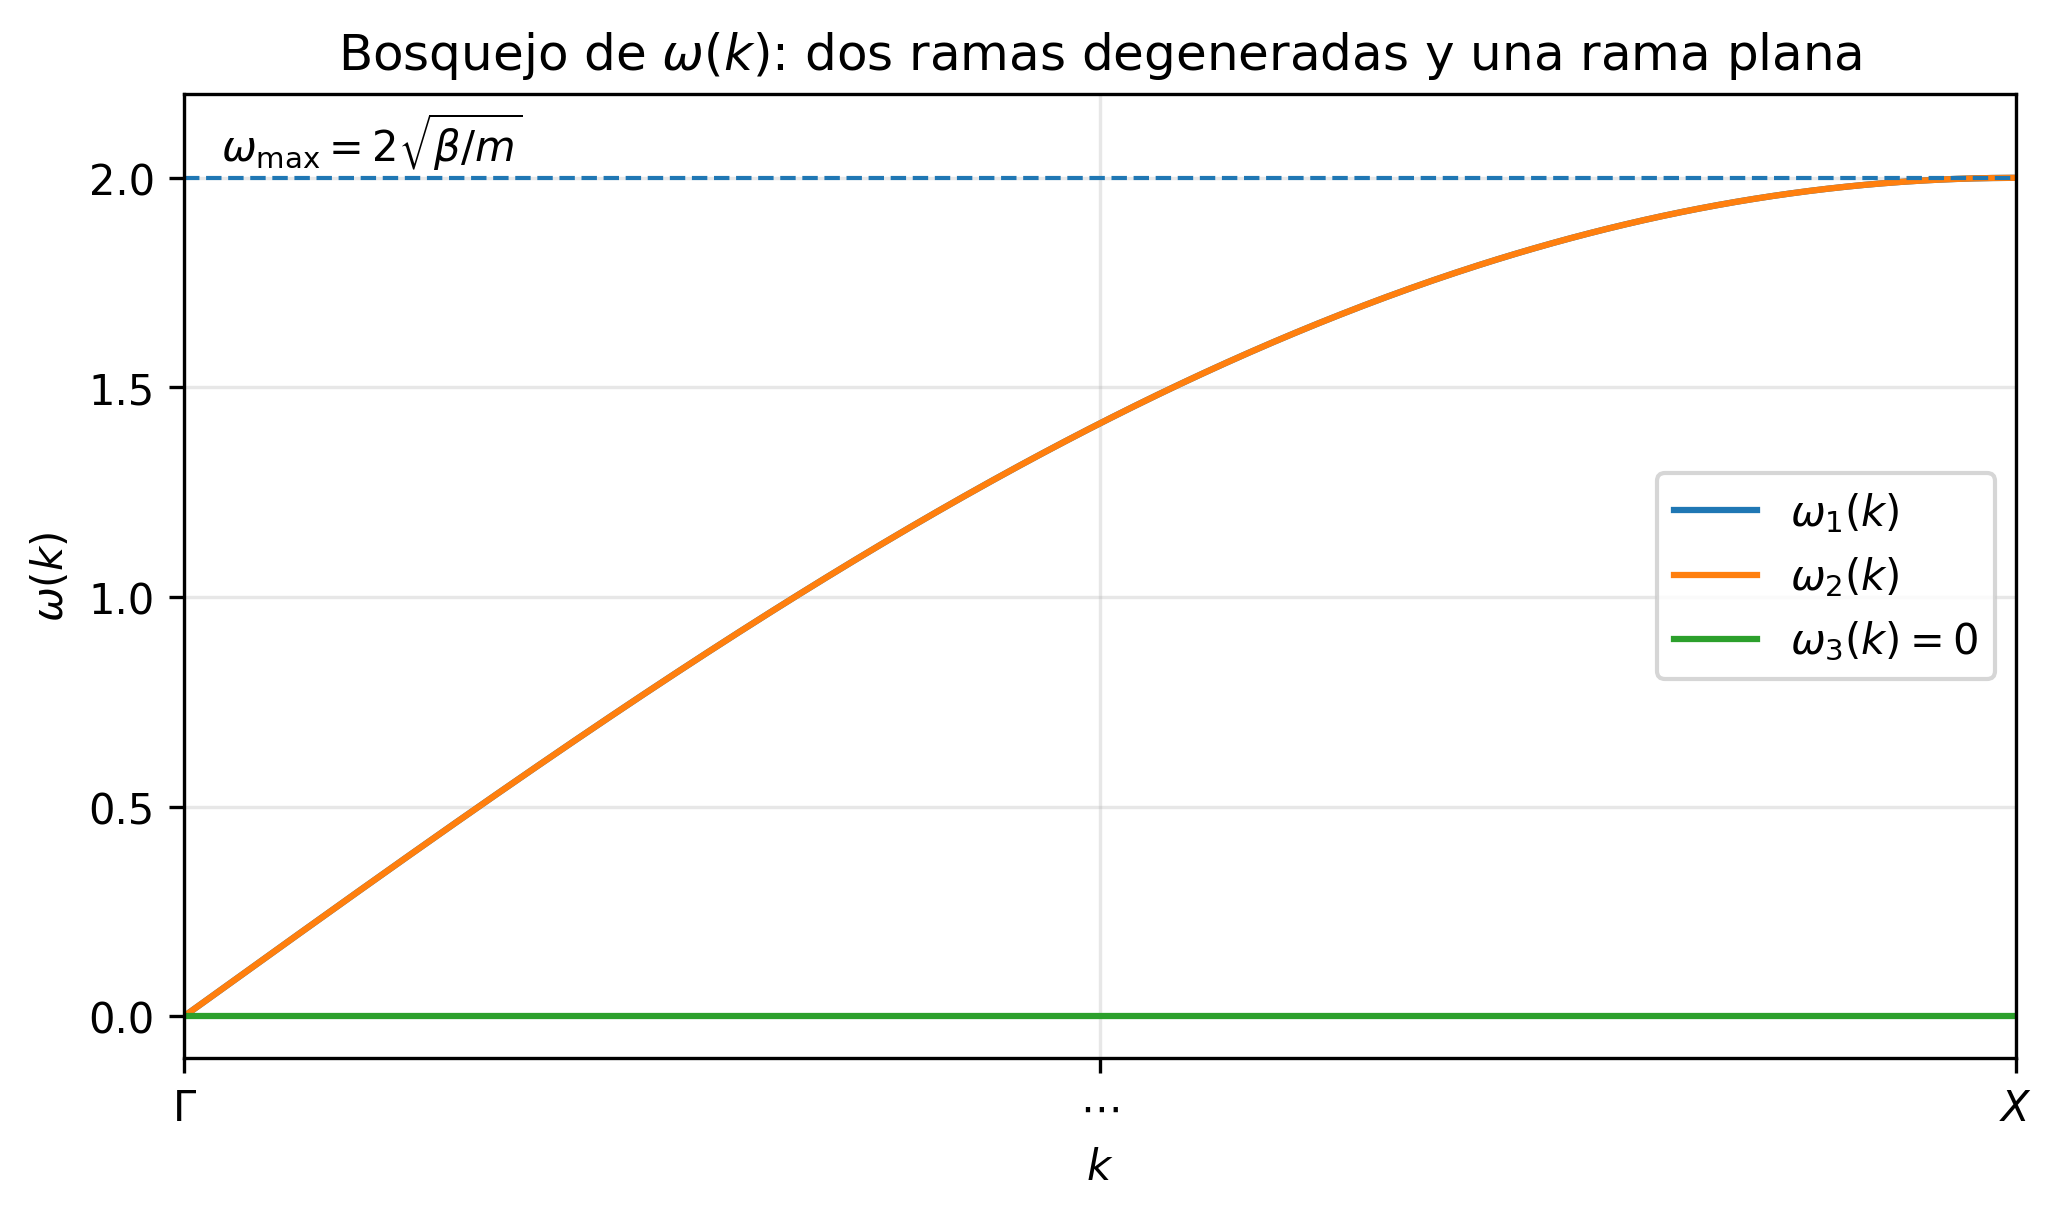
\includegraphics[width=0.9\textwidth]{dispersion_3_ramas.png}
    \caption{Bosquejo de la relación de dispersión \(\omega(k)\): dos ramas degeneradas y una rama plana.}
    \label{fig:dispersion_3_ramas}
\end{figure}

El diagrama de dispersión presenta dos ramas degeneradas que describen las vibraciones activas dentro del plano y una rama plana asociada a desplazamientos fuera del plano sin restauración.  
Esto refleja el comportamiento típico de una red cúbica simple con interacciones a primeros vecinos, donde solo dos direcciones responden dinámicamente a la propagación de la onda.


\fbox{\textbf{Inciso f)}}\;

Ahora que ya conocemos las tres relaciones de dispersión del inciso anterior, el siguiente paso consiste en identificar los \textbf{vectores propios} (o direcciones de vibración) asociados a cada una de ellas, y clasificar cuáles corresponden al \textbf{modo longitudinal} y cuáles a los \textbf{modos transversales}.

\medskip
Recordemos que el sistema de ecuaciones general es:
\[
\mathbf D(\vec k)\,\vec u = m\omega^2\,\vec u
\]
y para el caso particular \(\vec k = k\hat x + k\hat y\) la matriz dinámica tiene la forma:
\begin{equation}
\boxed{
\mathbf D(\vec k)=
\begin{pmatrix}
\Lambda & 0 & 0\\[2pt]
0 & \Lambda & 0\\[2pt]
0 & 0 & 0
\end{pmatrix}},
\qquad
\Lambda = 4\beta\,\sin^2\!\Big(\tfrac{ka}{2}\Big)
\label{eq:f_matriz_dinamica}
\end{equation}

De aquí obtenemos las tres ecuaciones escalares:
\begin{equation}
\Lambda\,u_x = m\omega^2\,u_x, 
\qquad
\Lambda\,u_y = m\omega^2\,u_y, 
\qquad
0 = m\omega^2\,u_z
\label{eq:f_ecuaciones_componentes}
\end{equation}

Estas tres ecuaciones nos dicen inmediatamente que:

\begin{itemize}
\item[$\bullet$] Las componentes \(u_x\) y \(u_y\) vibran con la misma frecuencia \(\omega^2 = \Lambda/m\)
\item[$\bullet$] Mientras que \(u_z\) no vibra (porque no hay fuerza restauradora en esa dirección).
\end{itemize}




\medskip
\textcolor{Tarawera}{\textbf{Modos en el plano \(x\text{–}y\)}}  
Dentro del plano, cualquier combinación de desplazamientos \((u_x,u_y,0)\) es posible,  
lo que significa que existe una \textbf{degeneración} de dos modos con la misma frecuencia.  
Para distinguirlos, es útil definir una base adaptada a la dirección del vector de onda.

Como el vector de onda es
\[
\vec k = k(\hat x + \hat y),
\]
podemos definir los siguientes tres vectores unitarios:
\begin{equation}
\boxed{
\hat e_L = \tfrac{1}{\sqrt2}(1,1,0),\qquad
\hat e_{T1} = \tfrac{1}{\sqrt2}(1,-1,0),\qquad
\hat e_{T2} = (0,0,1)
}
\label{eq:f_vectores_polarizacion}
\end{equation}


\begin{itemize}
\item[$\bullet$] \(\hat e_L\) apunta en la dirección de propagación de la onda (\(\vec k\))  
  y representa el \textbf{modo longitudinal}, donde los átomos se mueven en la misma dirección en que avanza la perturbación.
\item[$\bullet$] \(\hat e_{T1}\) está dentro del plano pero es perpendicular a \(\vec k\),  
  y corresponde a un \textbf{modo transversal en el plano}.\\
  \item[$\bullet$] \(\hat e_{T2}\) es perpendicular al plano, es decir, apunta a lo largo del eje \(z\);  
  representa el \textbf{modo transversal fuera del plano}.
\end{itemize}




\medskip
\textcolor{Tarawera}{\textbf{Sustituyendo en la ecuación de movimiento}}

Cada uno de estos vectores cumple:
\[
\mathbf D(\vec k)\,\hat e_i = m\omega_i^2\,\hat e_i
\]
de donde se obtiene:

\begin{equation}
\boxed{
\begin{aligned}
\omega_L^2(k)   &= \tfrac{4\beta}{m}\sin^2\!\Big(\tfrac{ka}{2}\Big)
&&\text{(modo longitudinal, paralelo a }\vec k\text{)}\\[4pt]
\omega_{T1}^2(k)&= \tfrac{4\beta}{m}\sin^2\!\Big(\tfrac{ka}{2}\Big)
&&\text{(modo transversal en el plano, }\perp\vec k\text{)}\\[4pt]
\omega_{T2}^2(k)&= 0
&&\text{(modo transversal fuera del plano, sobre }z\text{)}
\end{aligned}}
\label{eq:f_modos_frecuencias}
\end{equation}

\medskip

Los dos primeros modos (\(\hat e_L\) y \(\hat e_{T1}\)) tienen la misma frecuencia y, por tanto, son \textbf{degenerados}.  
  Ambos crecen con el mismo comportamiento senoidal:
  \[
  \omega(k) = 2\sqrt{\tfrac{\beta}{m}}\;\lvert\sin(\tfrac{ka}{2})\rvert
  \]
  
El tercer modo (\(\hat e_{T2}\)) no tiene frecuencia:  
  los átomos se mueven en la dirección \(z\) sin que los resortes ejerzan ninguna fuerza restauradora.  
  Es una rama \textbf{plana en cero}, típica de este tipo de modelos simplificados.

\medskip
Los tres vectores propios forman una base ortogonal natural para describir las vibraciones de la red:  
uno longitudinal y dos transversales, siendo estos últimos equivalentes dentro del plano y nulos fuera del mismo.  
En conjunto, describen por completo los \textbf{modos normales de vibración} de la red cúbica simple.






\end{document}
